\documentclass{article}

%\usepackage{natbib}
\usepackage[square,sort,comma,numbers]{natbib}
\usepackage{parskip}
\usepackage{multicol}
\usepackage{algorithm}
\usepackage{algpseudocode}
\usepackage{program}
\usepackage{listings} 
\usepackage{graphicx}
% \usepackage{amsmath}
% \usepackage{algorithm}
% \usepackage{algorithmic}

\begin{document}


\title{Parallelism and Performance}
\author{Patrick Collins}
\date{December 3, 2013}
\maketitle

% \begin{abstract}
% Abstract goes here...
% \end{abstract}

\section{Environment}
\subsection{Software}
\begin{itemize}
  \item Operating System: Ubuntu 13.10 Saucy
  \item Kernel: 3.11.0-13 generic x86\_64
  \item Compiler: GCC 4.8.1
  \end{itemize}
\subsection{Hardware}
\begin{itemize}
\item Processor: AMD FX-6300 Vishera
  \begin{itemize}
  \item Speed: 3.5 GHz (4.1 GHz Turbo)
  \item Cores: 6, one thread per core
  \item L1 Cache: 3 x 64 KB Instruction, 6x 16 KB Data
  \item L2 Cache 3x 2MB
  \item L3 Cache: 1x 8 MB
  \item Data width: 64 Bit
  \end{itemize}
\item Memory: 2 x 4 GB DDR3 1600 SDRAM
\end{itemize}


\section{Implementation}
For this project, I chose to pursue the multithreaded option. All of
the code in this section is single threaded, and so the POSIX command
\texttt{getrusage()} was used to measure CPU time of
exectuion. \texttt{getrrusage()} provides microsecond resolution for
all measurements, and is the most accurate way to measure performance
on Linux systems that implement it. Timer implementations tend to be
closely linked to hardware and the operating system, and so they vary
sigificantly from platform to platform. 

In the data that follows, the ``small'' size represents a run on an array of 1,000
\texttt{int}s, ``medium'' represents 10,000, and ``large'' represents
100,000. The following tests were run 100 times each, with 50
subprocesses running in paralell at any given time. Because these 50
processes did not consume all of the processes' resources, this parallelization did not
impact performance.

\subsection{Program Structure}
Prior to modifying the ``baseline code'' significantly, I attempted to
measure the impact on performance of some of the more mundane aspects
of writing C programs: namely the effect of different memory storage
durations and function calls on program performance. This was intended
to inform me as to whether or not it would be worthwhile to avoid
dynamically alocating memory, or to write macros in order to avoid
function calls.

\subsubsection{Storage Duration}

Before implementing any sorting algorithm, it is necessary to
determine the most effective way to store the data to be
sorted. The C11 standard defines four diferent storage durations:
static, automatic, thread and allocated (\cite[\S 6.2.4]{CStd}).
Thread variables are new in C11 and irrelevant for our purposes, since they cannot be
accessed from outside of the thread in which they are declared. That
leaves three candidate storage durations: static, automatic and
allocated. Memory with static duration is allocated either when a
variable is declared outside of a
function, or when a variable is declared inside of a function with the \texttt{static}
keyword. Automatic memory is allocated when a varaible is declared
inside of a function without the \texttt{static} keyword, and memory
with the `allocated` storage duration is allocated with the
\texttt{malloc()} function or similar. \smallskip

%types of memory? i don't know what language to use here
The C11 standard is silent, however, on how these different types of
memory are implemented. While allocated memory is most naturally
associated with the heap and automatic memory with the stack, the C11
standard does not contain the words ``stack'' or ``heap,'' leaving the
decision of how to implement each type to the compiler. In order to
determine the relative efficiencies of each type, then, it is
necessary to compare each on a realistic workload.

As a baseline, the single-threaded bubble sort was used to compare the
use of an integer array declared locally in the \texttt{main()}
function, an integer array declared in the global scope, and an
integer array allocated with the \texttt{malloc()} function. The
source code for each configuration is available in \texttt{bsort.c},
\texttt{bsort-global.c} and \texttt{bsort-malloc.c}. \bigskip

The results are as follows:
\begin{center}
\begin{tabular}{lllll}
 Implementation  &  Size & Average  &  Median     &  Standard Deviation             \\
 bsort           &  small    &  0.2238 s   &  0.2182 s            &  0.0093 s  \\
 bsort           &  medium   &  0.2220 s   &  0.2180 s            &  0.0085 s  \\
 bsort           &  large    &  23.4886 s  &  23.5006 s           &  0.6830 s  \\
 bsort global    &  small    &  0.2475 s   &  0.3389 s            &
 0.1960 s  \\
bsort global    &  large    &  30.6455 s  &  30.6182 s           &  0.4994 s  \\
 bsort global    &  medium   &  0.3068 s   &  0.3111 s            &  0.0131 s  \\
 bsort malloc    &  small    &  0.3429 s   &  0.4268 s            &  0.1703 s  \\
 bsort malloc    &  medium   &  0.3300 s   &  0.3306 s            &
 0.0132 s  \\
bsort malloc    &  large    &  32.0951 s  &  32.1063 s           &  0.4550 s  \\
\end{tabular}
\end{center}

This indicates that using an array stored in a local variable with automatic storage
duration provides a significant performance advantage over using
either a global variable or dynamically allocated memory.

% why do we care that they're not implemented with a stack?
\subsubsection{Function Call Overhead}
With some of the algorithms discussed later -- in particular,
quicksort and mergesort -- there is no way to avoid the overhead of
many function calls. In an iterative algorithm like bubble sort,
however, it is necessary to choose between inserting the code directly inside
the \texttt{main()} function or splitting it off into a separate
function. The C11 standard again does not specify that functions be
implemented with a stack (\cite[\S 6.7.6.3]{CStd}), although it does
include the \texttt{inline} keyword (\cite[\S 6.4.1, \S
6.7.4]{CStd}). The GCC Manual asserts that \texttt{inline} functions
are just as fast as writing a macro to manually inline the code in
question (\cite[\S 6.39]{GCCMan}).

A comparison of the three options is below:

\begin{center}
\begin{tabular}{lllll}
 Implementation  &  Average  & Size &  Median     &  Standard Deviation  \\
 bsort           &  small    &  0.2238 s   &  0.2182 s            &  0.0093 s  \\
 bsort           &  medium   &  0.2220 s   &  0.2180 s            &  0.0085 s  \\
 bsort           &  large    &  23.4886 s  &  23.5006 s           &  0.6830 s  \\
 bsort factored  &  small    &  0.1757 s   &  0.1966 s            &  0.1737 s  \\
 bsort factored  &  medium   &  0.2576 s   &  0.2586 s            &
 0.0056 s  \\
bsort factored  &  large    &  26.2215 s  &  26.1377 s           &  0.3313 s  \\
 bsort inline    &  small    &  0.1976 s   &  0.3117 s            &  0.1594 s  \\
 bsort inline    &  medium   &  0.2660 s   &  0.2668 s            &
 0.0026 s  \\
bsort inline    &  large    &  26.5490 s  &  26.5511 s           &  0.0266 s  \\
\end{tabular}
\end{center}

These figures do indicate a performance decrease after refactoring
the code to use a separate function for sorting. However, this is likely not a
measurement of the overhead of function calls, but rather the overhead
of dereferencing a pointer to the array each time. Changing to
reference implementation to use a pointer to modify the array inside
of the main function results in the following:

\begin{center}
\begin{tabular}{lllll}
 Implementation  &  Size    &  Average    &  Median     &  Standard Deviation  \\
 bsort pointer   &  small   &  0.1731 s   &  0.2046 s   &  0.1656 s            \\
 bsort pointer   &  medium  &  0.2685 s   &  0.2693 s   &  0.0031 s            \\
 bsort pointer   &  large   &  26.8550 s  &  26.8656 s  &  0.0692 s            \\
\end{tabular}
\end{center}

These measurements are identical to the measurements above from the
factored and inline versions, confirming that the slowdown is due to
the additional pointer. 

One possible solution to this is to copy the array into a local
variable at the start of the algorithm, perform the sorting on the
local variable, and then copy the local variable back into the
original array. This implementation resulted in the following speeds:

\begin{center}
\begin{tabular}{lllll}
 Implementation     &  Size    &  Average    &  Median     &  Standard Deviation  \\
 bsort pointer opt  &  medium  &  0.2723 s   &  0.2722 s   &  0.0061 s            \\
 bsort pointer opt  &  small   &  0.1892 s   &  0.2287 s   &  0.1796 s            \\
 bsort pointer opt  &  large   &  27.0129 s  &  26.9419 s  &  0.2426 s            \\
\end{tabular}
\end{center}

\subsubsection{Summary}
These measurements indicate that the optimal structuring of the
program is to use local, automatic variables to store the array to be
sorted whenever possible. They also indicate that refactoring code to remove the body of
the algorithm from the \texttt{main()} function is associated with
some overhead. However, this overhead is due to dereferencing the
pointer to the array to be sorted, rather than the function call
itself. This is not reduced by copying subsections of the data into a
static array inside of the algorithm.

\section{Sorting}
\subsection{Bubble Sort}
Information (source: \cite{Algos}):
\begin{itemize}
\item Average time complexity: $O(n^2)$ 
\item Average space complexity: $O(1)$ 
\end{itemize}

\subsubsection{Implementation}
Given by the project code. This is the reference sorting implementation.
\subsubsection{Performance}
Listed above. Average \texttt{int}s sorted per second sec are: 
\begin{center}
\begin{tabular}{lll}
 Implementation   & Size &  Average sorts/sec  \\
 bsort           &  1000   &  4.47 KSorts/sec \\
 bsort           &  10000   &  45.05 KSorts/sec \\
 bsort           &  100000    &  4.2 KSorts/sec\\
\end{tabular}
\end{center}

\subsection{Mergesort}
Information (source: \cite{Algos}):
\begin{itemize}
\item Average time complexity: $O(n\log n)$
\item Average space complexity: $O(1)$ 
\end{itemize}

A parallel mergesort was implemented as follows, using the
\texttt{pthreads.h} and \texttt{semaphore.h} libraries, compiled with
optimization level \texttt{-O3}:

\subsubsection{Implementation}
A \texttt{worker\_pool} struct was defined, consisting solely of a
semaphore and accessor methods to simplify the process of forking and
joining new threads when appropriate. Originally, the
\texttt{worker\_pool} struct used a semaphore to control access to an
\texttt{int} that listed the number of available worker threads, but
the time to synchronize access to the \texttt{int} was found to have
an unacceptably large impact on performance. 

At each level of recursion, the \texttt{mergesort} function requested
two threads from the worker pool, and started a parallel call to
\texttt{mergesort} for each thread that it received, executing the
remaining call(s) in the current thread. Afterwards, it blocked and
joined any threads that it started, then merged the area of the array
that was just sorted. Sorcecode is listed here:

\begin{lstlisting}[language=C]
void mergesort(int **array, int lo, int hi, worker_pool *wp)
{
	int mid = (hi + lo) / 2;
	pthread_t *th1, *th2;


	if (lo > hi){\begin{lstlisting}[language=C]

      return;
    }
    /* spin up a new thread to handle it if we can, */
    /* if not, continue in the current thread */
		
    
    if(!(th1 = start_worker(array, lo, mid, wp))){
      mergesort(array, lo, mid, wp);
    }

    if(!(th2 = start_worker(array, mid + 1, hi, wp))){
      mergesort(array, mid + 1, hi, wp);
    }

    /* block until as many threads return as necessary */
    if(th1){
      return_worker(wp, th1);
    }
    if(th2){
      return_worker(wp, th2);
    }
    
    merge(array, lo, mid, hi);
  }
}
\end{lstlisting}

\subsubsection{Performance}

In order to measure the speedup from parallelizing the sort, it was
necessary to move from measuring CPU time to wall
time. \texttt{clock\_getttime()} was used for this purpose, which
provided nanosecond resolution. The sizes of arrays were redefined
because it was impossible to get meaningful measurements from the
bubblesort-sized arrays. ``large'' represents $2^{22}$ elements,
``xlarge'' represents $2^{24}$ elements, and ``xxlarge'' represents
$2^{28}$. Smaller sizes were measured -- $2^{14}$ and $2^{18}$ --
however, these sorts completed too quickly to yield meaningful data.

The table below lists the runtime of the algorithm for a number of
different threadcounts at a number of different sizes. The optimum
number of threads at each size has been listed in \textbf{bold}. 50
runs were conducted at each size. 

\begin{center}
\begin{tabular}{lllll}
 Threads    &  Size     &  Average    &  Median     &  Standard Deviation  \\
 2   &  large    &  0.1848 s   &  0.0000 s   &  0.3289 s            \\
 4   &  large    &  0.1428 s   &  0.0000 s   &  0.3051 s            \\
 6   &  large    &  0.1625 s   &  0.0000 s   &  0.3252 s            \\
 8   &  large    &  0.1605 s   &  0.0000 s   &  0.3215 s            \\
 \textbf{10}  & \textbf{large}    & \textbf{0.1408 s}   &  \textbf{0.0000 s}   &  \textbf{0.3012 s}            \\
 12  &  large    &  0.1546 s   &  0.0000 s   &  0.3115 s            \\
 14  &  large    &  0.1600 s   &  0.0000 s   &  0.3203 s            \\
 16  &  large    &  0.1768 s   &  0.0000 s   &  0.3332 s            \\
 18  &  large    &  0.1701 s   &  0.0000 s   &  0.3211 s            \\
 20  &  large    &  0.2001 s   &  0.0000 s   &  0.3382 s            \\
 22  &  large    &  0.1822 s   &  0.0000 s   &  0.3248 s            \\
 24  &  large    &  0.1940 s   &  0.0000 s   &  0.3280 s            \\
 26  &  large    &  0.1757 s   &  0.0000 s   &  0.3137 s            \\
 28  &  large    &  0.1973 s   &  0.0000 s   &  0.3176 s            \\
 30  &  large    &  0.2003 s   &  0.0000 s   &  0.3235 s            \\
 32  &  large    &  0.2331 s   &  0.0000 s   &  0.3281 s            \\
 34  &  large    &  0.2236 s   &  0.0000 s   &  0.3173 s            \\
 36  &  large    &  0.1976 s   &  0.0000 s   &  0.3046 s            \\
 38  &  large    &  0.1944 s   &  0.0000 s   &  0.3000 s            \\
 2   &  xlarge   &  3.4553 s   &  3.0593 s   &  0.5155 s            \\
 4   &  xlarge   &  2.9820 s   &  3.0000 s   &  0.4822 s            \\
 6   &  xlarge   &  2.3354 s   &  2.1687 s   &  0.3722 s            \\
 8   &  xlarge   &  2.3066 s   &  2.2245 s   &  0.3759 s            \\
 10  &  xlarge   &  2.4475 s   &  2.4179 s   &  0.5019 s            \\
\textbf{12}  & \textbf{xlarge}   &  \textbf{2.2937 s}   &  \textbf{2.0000 s}   &  \textbf{0.4411 s}            \\
 14  &  xlarge   &  2.5491 s   &  2.3162 s   &  0.5451 s            \\
 16  &  xlarge   &  2.9614 s   &  3.0000 s   &  0.5531 s            \\
 18  &  xlarge   &  3.1358 s   &  3.0000 s   &  0.4826 s            \\
 20  &  xlarge   &  3.1215 s   &  3.0643 s   &  0.6395 s            \\
 22  &  xlarge   &  3.1138 s   &  3.0933 s   &  0.7993 s            \\
 24  &  xlarge   &  3.2745 s   &  3.2388 s   &  0.9116 s            \\
 26  &  xlarge   &  2.7170 s   &  2.3227 s   &  0.8581 s            \\
 28  &  xlarge   &  2.9161 s   &  2.3688 s   &  1.0347 s            \\
 30  &  xlarge   &  3.0384 s   &  2.4190 s   &  1.2166 s            \\
 32  &  xlarge   &  2.9279 s   &  3.0000 s   &  0.9387 s            \\
 34  &  xlarge   &  3.0896 s   &  3.0000 s   &  0.7827 s            \\
 36  &  xlarge   &  3.5687 s   &  3.2937 s   &  0.9186 s            \\
 38  &  xlarge   &  3.4553 s   &  3.0626 s   &  0.7782 s            \\
 16  &  xxlarge  &  13.2893 s  &  13.0762 s  &  0.9961 s            \\
 18  &  xxlarge  &  14.0146 s  &  14.0141 s  &  0.9845 s            \\
 20  &  xxlarge  &  13.9357 s  &  14.0421 s  &  1.8193 s            \\
 22  &  xxlarge  &  12.9159 s  &  13.0000 s  &  2.1564 s            \\
 24  &  xxlarge  &  11.5415 s  &  11.0000 s  &  2.2646 s            \\
 \textbf{26}  &  \textbf{xxlarge}  &  \textbf{11.4277 s}  &  \textbf{10.0000 s}  &  \textbf{2.6742 s}            \\
 28  &  xxlarge  &  12.3660 s  &  11.0000 s  &  3.0040 s            \\
 30  &  xxlarge  &  12.3035 s  &  11.0000 s  &  2.7740 s            \\
 34  &  xxlarge  &  14.3556 s  &  13.0000 s  &  2.9419 s            \\
 36  &  xxlarge  &  14.0130 s  &  13.3280 s  &  2.2762 s            \\
\end{tabular}
\end{center}

It is important to note  that the error increases as the number
of threads and the array size increases. This is likely due to the fact that the heaviest
workloads were able to make full use of all six cores -- therefore,
the performance of the algorithm was directly impacted by the
operating system's decisions to allocate resources to or from its
operation. The optimum number of threads is also proportional to the
number of elements measured. This likely reflects the fact that the
additional overhead of stopping and starting each thread becomes
relatively less important as the amount of work done by each thread increases.

\subsubsection{Summary}
The figures below are listed for the best performance within each size
category, the bolded entries above.
\begin{center}
\begin{tabular}{lll}
 Implementation   & Size &  Average sorts/sec  \\
 mergesort par &     4194304   &  29.79 MSorts/sec \\
 mergesort par           &  67108864   &  29.26 MSorts/sec \\
 mergesort par           &  100000    &  23.49 MSorts/sec\\
\end{tabular}
\end{center}

\subsection{Counting Sort}
Information (source: \cite{Algos}):
\begin{itemize}
\item Average time complexity: $O(n \times k)$
\item Average space complexity: $O(1)$ 
\end{itemize}

\subsubsection{Implementation}

The code provided in the reference implementation generated numbers to
fill the array with the following code:
\begin{lstlisting}[language=C]
  for (int i = 0; i < size; i++){ 
    array[i] = (i << 6) \% (17 * 17);
  }
\end{lstlisting}
  
This implies that values in the generated arrays are restricted to the
range [0\ldots289], with the exception of integer overflows resulting
in some random numbers. This code was changed to
\begin{lstlisting}[language=C]
  for (int i = 0; i < size; i++){ 
    array[i] = ((unsigned)(i << 6)) \% (17 * 17));
  }
\end{lstlisting}

in order to avoid signed integer overflow, which is undefined by the C
standard. 

The small range of values was exploited by an implementation of
counting sort. As a non-comparative sort, counting sort has a
substantially lower algorithmic time complexity than either mergesort
or bubblesort -- it is linear on the size of the input array. The
algorithm is also extremely easy to implement:

\begin{lstlisting}[language=C]
int tmp[RANGE] = {0}; 

void populate_tmp(int *array, int n)
{
	for(int i = 0; i < n; i++){
		tmp[array[i]]++;
	}
}

void unroll_tmp(int *array, int range)
{
	int counter = 0;
	for(int i = 0; i < range; i++){
		while(tmp[i]--){
			array[counter++] = i;
		}
	}
}

void csort(int *array, int size)
{
	populate_tmp(array, size);
	unroll_tmp(array, RANGE);
}
\end{lstlisting}

A parallel version was implemented by dividing the array to be sorted
into a number of chunks equal to the number of worker
threads. However, this introduced the possibility of synchronization
errors due to multiple threads accessing the \texttt{tmp} array at the
same time, so the GCC built-in atomic operations were used as follows: 

\begin{lstlisting}[language=C]
void populate_tmp(int **array, int start, int end)
{
	for(int i = start; i < end; i++){
		__sync_fetch_and_add(&tmp[(*array)[i]], 1);
	}
}
\end{lstlisting}

in order to avoid this problem. However, this implementation was found
to be unacceptably slow (see performance, below). Because of earlier results regarding the
speed of access to \texttt{sem\_t} objects, an alternate
implementation was used that defined \texttt{tmp} as an array of
\texttt{sem\_t}s and the \texttt{sem\_post()} operation was used to
increment them instead. 

\subsubsection{Performance}
The sizes used here are the same as above in the \texttt{mergesort}
section, except for the introduction of a new size, ``xxxlarge'',
equal to $2^{30}$. With the 32 bit integers implemented on this
computer, this array represented 4 GB of input data -- half of the
machine's memory. Larger sizes were attempted, but the operating
system became nonresponsive as it was forced to push data onto the
pagefile. 20 runs were performed for each entry listed. For parallel
implementations, the number of threads is listed beside the name.

\begin{center}
\begin{tabular}{lllll}
 Implementation  &  Size      &  Average   &  Median    &  Standard Deviation  \\
 sem\_t 4        &  xlarge    &  1.2769 s  &  1.3795 s  &  0.2075 s            \\
 sem\_t 6        &  xlarge    &  1.2205 s  &  1.0000 s  &  0.3378 s            \\
 sem\_t 8        &  xlarge    &  1.2672 s  &  1.0000 s  &  0.3652 s            \\
 atomic add 4    &  xlarge    &  4.1434 s  &  4.0000 s  &  0.5776 s            \\
 atomic add 6    &  xlarge    &  4.1936 s  &  4.0000 s  &  0.2171 s            \\
 atomic add 8    &  xlarge    &  4.2367 s  &  4.2004 s  &  0.2412 s            \\
 sequential      &  xlarge    &  0.2354 s  &  0.0000 s  &  0.3595 s            \\
 sem\_t 4        &  xxlarge   &  5.1712 s  &  5.2269 s  &  0.1334 s            \\
 sem\_t 6        &  xxlarge   &  4.5868 s  &  4.2496 s  &  0.5785 s            \\
 sem\_t 8        &  xxlarge   &  4.2125 s  &  4.2479 s  &  0.1451 s            \\
 sequential      &  xxlarge   &  0.1174 s  &  0.1310 s  &  0.0395 s            \\
 sequential      &  xxxlarge  &  3.2424 s  &  3.0000 s  &  0.2681 s            \\
\end{tabular}
\end{center}

For a sorting algorithm as efficient as counting sort, the cost of
synchronization outweighed the benefits of parallelism. The sequential
version consistently outperformed the other implementations by an
order of magnitude. 

\subsubsection{Performance}
Average \texttt{int}s sorted per second sec are: 

\begin{center}
\begin{tabular}{lllll}
 Implementation  &  Size      &  Average sorts/sec \\
 sem\_t 4        &  xlarge    &  52.56 MSorts/sec \\
 sem\_t 6        &  xlarge    &  54.98 MSorts/sec \\
 sem\_t 8        &  xlarge    &  52.95 MSorts/sec \\
 atomic add 4    &  xlarge    &  16.20 MSorts/sec \\
 atomic add 6    &  xlarge    &  16.00 MSorts/sec \\
 atomic add 8    &  xlarge    &  15.83 MSorts/sec \\
 \textbf{sequential}      &  \textbf{xlarge}    &  \textbf{285.08 MSorts/sec} \\
 sem\_t 4        &  xxlarge   &  51.91 MSorts/sec \\
 sem\_t 6        &  xxlarge   &  58.52 MSorts/sec \\
 sem\_t 8        &  xxlarge   &  63.72 MSorts/sec \\
 \textbf{sequential}      &  \textbf{xxlarge}   &  \textbf{2.286 GSorts/sec} \\
 \textbf{sequential}      &  \textbf{xxxlarge}  &  \textbf{331.16 MSorts/sec} \\
\end{tabular}
\end{center}

\subsection{Matrix-Matrix Multiply}
\begin{itemize}
\item Average time complexity: $O(n^3)$
\item Average space complexity: $O(1)$ 
\end{itemize}

\subsubsection{Implementation}
OpenMP was used to paralellize the matrix multiplication.

The original code provided for the project multiplied one square
matrix with itself. Like the earlier array initialization algorithm
provided, it deterministically initialized the matrix with with values
inside of a small range. This fact was again exploited to provide for
maximum cache locality. The algorithm was left unmodified as a triple
for-loop, and all code was compiled at -O3 optimization level.

The initial optimization made was to transpose a copy the
\texttt{first} matrix for multiplication, so that the data would be
stored in column-major order. However, it was noted that the
pseudo-random number generation algorithm provided only produced
symmetric matrices, and so, rather than copy the \texttt{first}
matrix into a separate region of memory, the multiplication was simply
performed with the \texttt{first} matrix serving as a transposed copy
of itself. 

This reduced the total amount of data involved in the calculation to
$8 n^2$. For matrix multiplications involving less than $1000^2$
elements, then, this allowed all of the data to be fit into the L2
cache of the processor. This resulted in an extremely large speedup
for matrices at or below this size. 

Next, parallelism was introduced, increasing the gains due to cache
locality. A number of different configurations in OpenMP were
tested. The most effective parallelization of multiplication was found
to be the following (get\_cell is an inline function that selects the
appropriate element from a matrix with pointer arithmetic):

\begin{lstlisting}[language=C]
void multiply_matrix_symm_transp(int *first, int *result, int size)
{
  register int c, d, k;
  int *arow, *brow, *ans;
#pragma omp parallel for shared(first, result, ans) \
  private(c, d, k, arow, brow)
  for ( c = 0 ; c < size ; c++ )
  {
    for ( d = 0 ; d < size ; d++ )
    {
      arow = get_cell(first, c, 0, size);
      brow = get_cell(first, d, 0, size);
      ans = get_cell(result, c, d, size);
      for ( k = 0 ; k < size; k++ )
      {
        ans += *(arow + k) * *(brow + k);
      }
    }
  }
}
\end{lstlisting}


\subsubsection{Performance}
Below, the sequential and parallel implementations' performances are
listed side by side. 20 runs were conducted at each size for each program.
\begin{center}
\begin{tabular}{lrlll}
 Implementation  &  Size (n)  &  Average   &  Median    &  Standard Deviation  \\
 sequential       &       100  &  3.6504 s  &  2.2446 s  &  3.0339 s            \\
 \textbf{parallel}       &       100  &  0.0000 s  &  0.0000 s  &  0.0000 s            \\
 sequential       &       500  &  3.5555 s  &  2.2974 s  &  2.7335 s            \\
\textbf{parallel}      &       500  &  0.0481 s  &  0.0000 s  &  0.2095 s            \\
 sequential       &       750  &  3.7585 s  &  2.3011 s  &  2.4344 s            \\
 \textbf{parallel}       &       750  &  0.1331 s  &  0.0000 s  &  0.3168 s            \\
 sequential       &      1000  &  3.8744 s  &  2.5344 s  &  2.9490 s            \\
 \textbf{parallel}       &      1000  &  0.2529 s  &  0.0000 s  &  0.2833 s            \\
 \textbf{sequential}       &      2000  &  3.8076 s  &  2.2067 s  &  2.6520 s            \\
 parallel       &      2000  &  3.1426 s  &  3.0000 s  &  0.5568 s            \\
 \textbf{sequential}       &      3000  &  3.7991 s  &  3.0266 s  &  1.7908 s            \\
 parallel       &      3000  &  7.6652 s  &  8.0000 s  &  0.5213 s            \\
\end{tabular}
\end{center}

Multithreading introduced massive gains -- with speedups larger than
10x -- for matrices of less than $1000 \times 1000$ elements. However, relative
performance degraded rapidly above this threshold. This was likely
caused by the size of the two matrices exceeding the size of the L2
cache. 


An analysis with cachegrind shows that the parallel version made
more data references than the sequential by an order of magnitude.

Sequential:
\begin{verbatim}
 D   refs:      3,001,450,864  (3,000,122,877 rd   + 1,327,987 wr)
 D1  misses:    1,189,838,966  (1,188,773,231 rd   + 1,065,735 wr)
 LLd misses:          128,476  (        2,117 rd   +   126,359 wr)
 D1  miss rate:          39.6% (         39.6%     +      80.2%  )
 LLd miss rate:           0.0% (          0.0%     +       9.5%  )
 
 LL refs:       1,189,839,977  (1,188,774,242 rd   + 1,065,735 wr)
 LL misses:           129,464  (        3,105 rd   +   126,359 wr)
 LL miss rate:            0.0% (          0.0%     +     % 9.5%  )
\end{verbatim}

Parallel:
\begin{verbatim}
 D   refs:       54,129,593,701  (54,082,303,124 rd   + 47,290,577 wr)
 D1  misses:      3,397,260,441  ( 3,378,724,797 rd   + 18,535,644 wr)
 LLd misses:      1,442,441,761  ( 1,441,866,257 rd   +    575,504 wr)
 D1  miss rate:             6.2% (           6.2%     +       39.1%  )
 LLd miss rate:             2.6% (           2.6%     +        1.2%  )
 
 LL refs:         3,397,261,675  ( 3,378,726,031 rd   + 18,535,644 wr)
 LL misses:       1,442,442,966  ( 1,441,867,462 rd   +    575,504 wr)
 LL miss rate:              0.5% (           0.5%     +        1.2%  )
\end{verbatim}

The sequential version had a substantially higher miss rate on the L1
data cache. It also appears that the operating system was able to
prefetch both of the matrices, eliminating L2 misses entirely. On the
other hand, the non-sequential access pattern used by OpenMP appears
to have defeated the prefetch buffer and caused L2 cache misses,
resulting in the severe loss in performance that was observed.

\section{Conclusion}
All code is available on the Github repository
https://github.com/capitalsigma/cmsc222-optimization.

Having examined the impact of multithreading on performance in a
variety of different situations and implementations, the question
remains: how much more performance can be gained through the addition
of more threads and more cores?

The data collected do not, on the whole, support any one clear
answer. It appears that secondary factors like choice of algorithm and
cache capacity dominate in most situations. Furthermore, the
performance benefit of each additional thread has rarely proven to be
linear. The best data collected in order to perform this comparison,
however, is likely the parallel mergesort data. Below is a graph of
the percentage improvement per additional thread used in the mergesort
algorithm, relative to the singlethreaded version ($1 -(t_n \div
t_1)$):

\DeclareGraphicsExtensions{.png}
\begin{center}
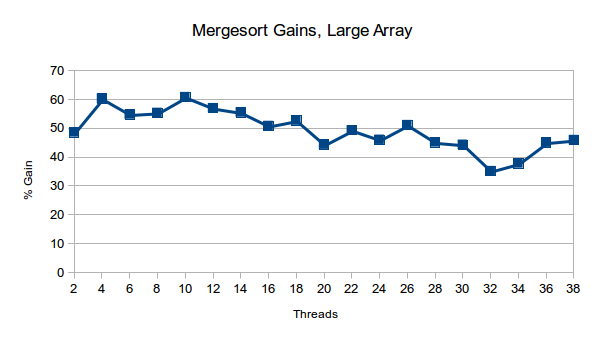
\includegraphics{gains-large.png}
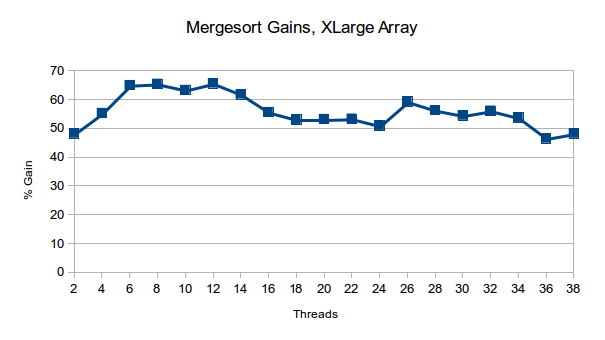
\includegraphics{gains-xlarge-nolegend.png}
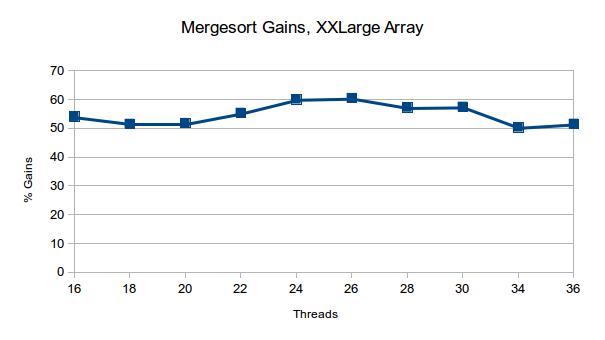
\includegraphics{gains-xxlarge-nolegend.png}
\end{center}

The data demonstrate that merely extending the program to more threads
is not an effective method of increasing performance: each achieves a
maximum at some particular threadcount and then declines. The
particular threadcount at which the maximum speed is achieved also
varies for each array size. Assuming that the ideal configuration is
expressible in terms of threads per core, we arrive at the following
approximations regarding the \% performance gain per thread-core
under ideal circumstances:

\begin{eqnarray*}
&\textrm{Gain/thread $\times$ core}_{\textrm{size}} =& \frac {\textrm{max
    gain} * \textrm{cores}} {\textrm{optimum threads}}\\
&\textrm{Gain/thread $\times$ core}_\textrm{large} =& 36.513\%\\
&\textrm{Gain/thread $\times$ core}_\textrm{xlarge} =& 32.810\%\\
&\textrm{Gain/thread $\times$ core}_\textrm{xxlarge} =& 13.867\%\\
\end{eqnarray*}

The last measurement is likely an outlier, as the dataset for the
xxlarge array size is less complete. The previous two measurements
appear to agree, however: at the point of maximum performance gain,
integer sorting occurs approximately 30\% faster per thread per core
in a multithreaded environment than in a singlethreaded
one. 


\bibliography{writeup}
\bibliographystyle{acm}
\nocite{*}


\end{document}